\documentclass{tixtex}
\hypersetup{pdftitle={St. Nicholas residences -- or: baycentric subdivision}}
            
\usetikzlibrary{calc}

\tikzset{%
    Dpoint/.style={shape=circle,fill=#1,inner sep=1.3pt}, Dpoint/.default={blue},
    Dshapefillgray/.style={fill=black!40, fill opacity=0.2},
    Dline/.style={line width=0.7pt, line join=bevel}
}

%%%%%%%%%%%%%%%%%%%%%%%%%%%%%%%%%%%%%%%%%%%%%%%%%%%%%%%%%%%%%%%%%%%%%%%%%%%

% As a motivating example, here is a simple macro that takes three
% coordinates and draws the (first) barycentric subdivision of the
% triangle defined by those points. (See below for examples.)
%
\newcommand{\subdiv}[3]{
    % calculate barycenters ("centroids")
    \path
        (barycentric cs:#1=1,#2=1) coordinate (m3)
        (barycentric cs:#2=1,#3=1) coordinate (m1)
        (barycentric cs:#1=1,#3=1) coordinate (m2)
        (barycentric cs:#1=1,#2=1,#3=1) coordinate (mM);
    
    % draw 2-simplex ("filled triangle")
    % and boundary 1-simplices ("lines")
    \draw [Dshapefillgray,Dline] (#1)--(#2)--(#3)--cycle;
    
    % draw 1-simplices ("lines") of subdivision
    \foreach \c in {#1,#2,#3,m1,m2,m3}
        \draw [Dline] (\c)--(mM);
    
    % draw 0-simplices ("points")
    \foreach \c in {#1,#2,#3,m1,m2,m3,mM}
        \path (\c) node [Dpoint] {};
}

%%%%%%%%%%%%%%%%%%%%%%%%%%%%%%%%%%%%%%%%%%%%%%%%%%%%%%%%%%%%%%%%%%%%%%%%%%%

% And here is the fully recursive version of the above, i. e.
% \subdivrec{A}{B}{C}{n} draws the n-th barycentric subdivision
% of the triangle defined by the coordinates (A),(B) and (C).
%
\makeatletter
\newcommand{\subdivrec}[4]{
    \ifnum#4 < 1 % recursion level 0: draw simplex
        
        % draw 2-simplex and boundary 1-simplices
        \draw [Dshapefillgray,Dline] (#1)--(#2)--(#3)--cycle;
    
        % draw 0-simplices
        \foreach \@c in {#1,#2,#3}
            \path (\@c) node [Dpoint] {};
        
    \else % non-zero recursion level: calculate again and recurse
        
        % calculate barycenters
        \path
            (barycentric cs:#1=1,#2=1) coordinate (m3r#4)
            (barycentric cs:#2=1,#3=1) coordinate (m1r#4)
            (barycentric cs:#1=1,#3=1) coordinate (m2r#4)
            (barycentric cs:#1=1,#2=1,#3=1) coordinate (mMr#4);
        
        \begingroup
        \pgfmathtruncatemacro{\@reclevel}{#4-1} % decrement recursion level
        \foreach \@cA/\@cB/\@cC in
                {#1/m2r#4/mMr#4,   #1/m3r#4/mMr#4,
                 #2/m1r#4/mMr#4,   #2/m3r#4/mMr#4,
                 #3/m1r#4/mMr#4,   #3/m2r#4/mMr#4}
            % edef trick to expand arguments for \subdivrec
            \edef\zz{\noexpand\subdivrec{\@cA}{\@cB}{\@cC}{\@reclevel}}\zz;
        \endgroup
    \fi
}
\makeatother

% We can use \subdivrec to draw a "Haus vom Nikolaus"
% ( http://de.wikipedia.org/wiki/Haus_vom_Nikolaus )
% in its n-th barycentric subdivision.
%
\newcommand{\nikolausresidenz}[1]{
    \begingroup
    
    \newcommand{\xx}{14}
    \newcommand{\yy}{14}
    \newcommand{\xxh}{7}
    \newcommand{\yyh}{7}
    \newcommand{\yyt}{21}
    
    \path
        (0,0)       coordinate (Nld)
        (\xx,0)     coordinate (Nrd)
        (\xx,\yy)   coordinate (Nru)
        (0,\yy)     coordinate (Nlu)
        (\xxh,\yyh) coordinate (Nm)
        (\xxh,\yyt) coordinate (Nt)
    ;
        
    \foreach \cA/\cB/\cC in 
            {Nld/Nrd/Nm,    Nld/Nlu/Nm,
             Nrd/Nru/Nm,    Nru/Nlu/Nm,
             Nlu/Nru/Nt}
        \subdivrec{\cA}{\cB}{\cC}{#1};
        
    \endgroup
}

%%%%%%%%%%%%%%%%%%%%%%%%%%%%%%%%%%%%%%%%%%%%%%%%%%%%%%%%%%%%%%%%%%%%%%%%%%%

\begin{document}
Motivating examples using \verb|\subdiv|:
\begin{center}
    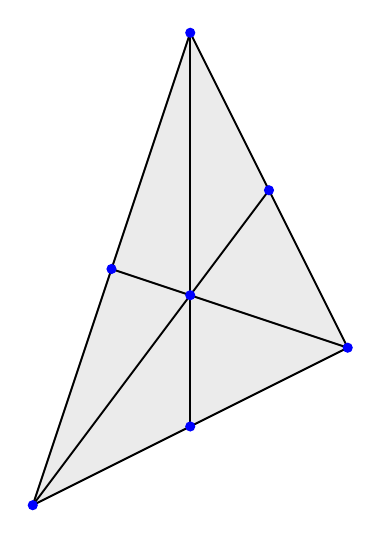
\begin{tikzpicture}[scale=2]
        \path
            (0,3) coordinate (A)
            (-1,0) coordinate (B)
            (1,1) coordinate (C);
            
        \subdiv{A}{B}{C}
    \end{tikzpicture}
    %
    \hspace{3cm}
    %
    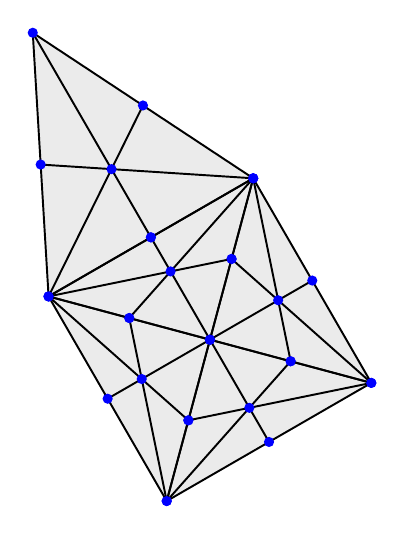
\begin{tikzpicture}[scale=1.5,rotate=30]
        \path
            (0,0) coordinate (Nld)
            (2,0) coordinate (Nrd)
            (2,2) coordinate (Nru)
            (0,2) coordinate (Nlu)
            (1,1) coordinate (Nm)
            (1,4) coordinate (Nt);
            
        \foreach \cA/\cB/\cC in 
                {Nld/Nrd/Nm,    Nld/Nlu/Nm,
                 Nrd/Nru/Nm,    Nru/Nlu/Nm,
                 Nlu/Nru/Nt}
            \subdiv{\cA}{\cB}{\cC};
            
    \end{tikzpicture}
\end{center}

%%%%%%%%%%%%%%%%%%%%%%%%%%%%%%%%%%%%%%%%%%%%%%%%%%%%%%%%%%%%%%%%%%%%%%%%%%%

\vspace{3cm}

Now we use \verb|\subdivrec| to draw the second barycentric
subdivision of a triangle (i.\,e. the barycentric subdivision of its
barycentric subdivision):
\begin{center}
    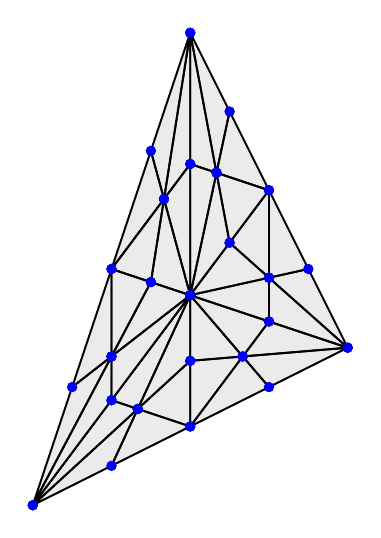
\begin{tikzpicture}[scale=2]
        \path
            (0,3) coordinate (A)
            (-1,0) coordinate (B)
            (1,1) coordinate (C);
            
        \subdivrec{A}{B}{C}{2}
    \end{tikzpicture}
\end{center}

\newpage
%
In Germany we have a riddle for children:
draw a ``Haus vom Nikolaus''\footnote{%
    \url{http://de.wikipedia.org/wiki/Haus_vom_Nikolaus}}
(house of St.~Nicholas) without lifting the pen from the paper and without
drawing any line twice. Mathematically put: find an Eulerian path in the
following graph:
\begin{center}
    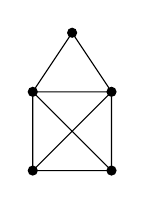
\begin{tikzpicture}[scale=0.5]
        \path
            (0,0) coordinate (Nld)
            (2,0) coordinate (Nrd)
            (2,2) coordinate (Nru)
            (0,2) coordinate (Nlu)
            (1,3.5) coordinate (Nt);
        \draw (Nld)--(Nlu)--(Nt)--(Nru)--(Nlu)--(Nrd)--(Nru)--(Nld)--(Nrd);
        \foreach \c in {Nld,Nrd,Nru,Nlu,Nt}
            \path (\c) node [Dpoint=black] {} ;
    \end{tikzpicture}
\end{center}
(note that there is \emph{not} a graph vertex at the intersection of the
two diagonal lines).

Now we put an extra vertex at the crossing in the middle and interpret the
figure as a composition of five 2-simplices (``filled triangles'').
Then resulting complex in its $n$-th barycentric subdivision can be drawn
via \verb|\nikolausresidenz{n}|:
\begin{center}
    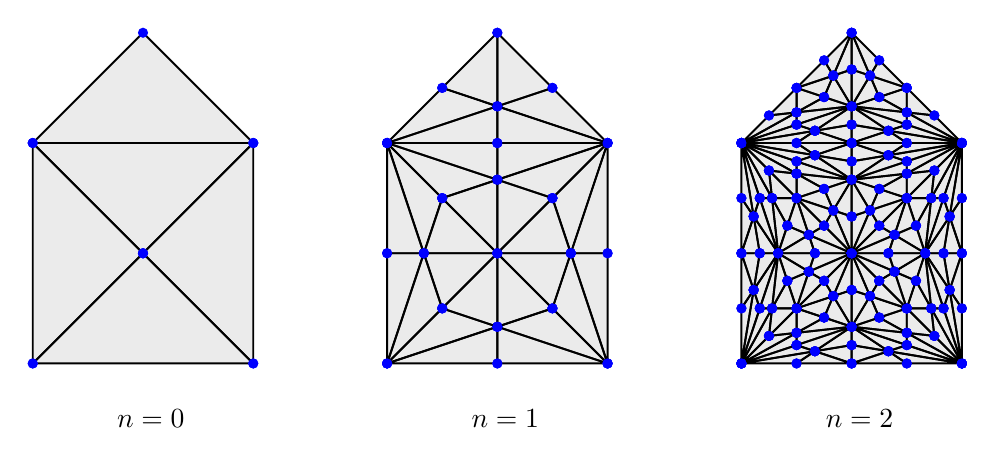
\begin{tikzpicture}
        \foreach \n in {0,...,2} {
            \begin{scope}[shift={($(4.5*\n,0)$)},scale=0.2]
                \expandafter\nikolausresidenz\n
            \end{scope}
            \path ($(4.5*\n+1.5,-0.7)$) node {$n=\n$};
        };
    \end{tikzpicture}
\end{center}

\bigskip
\verb|\nikolausresidenz{3}| on the next page:

\newpage\enlargethispage{2cm}
\begin{center}
    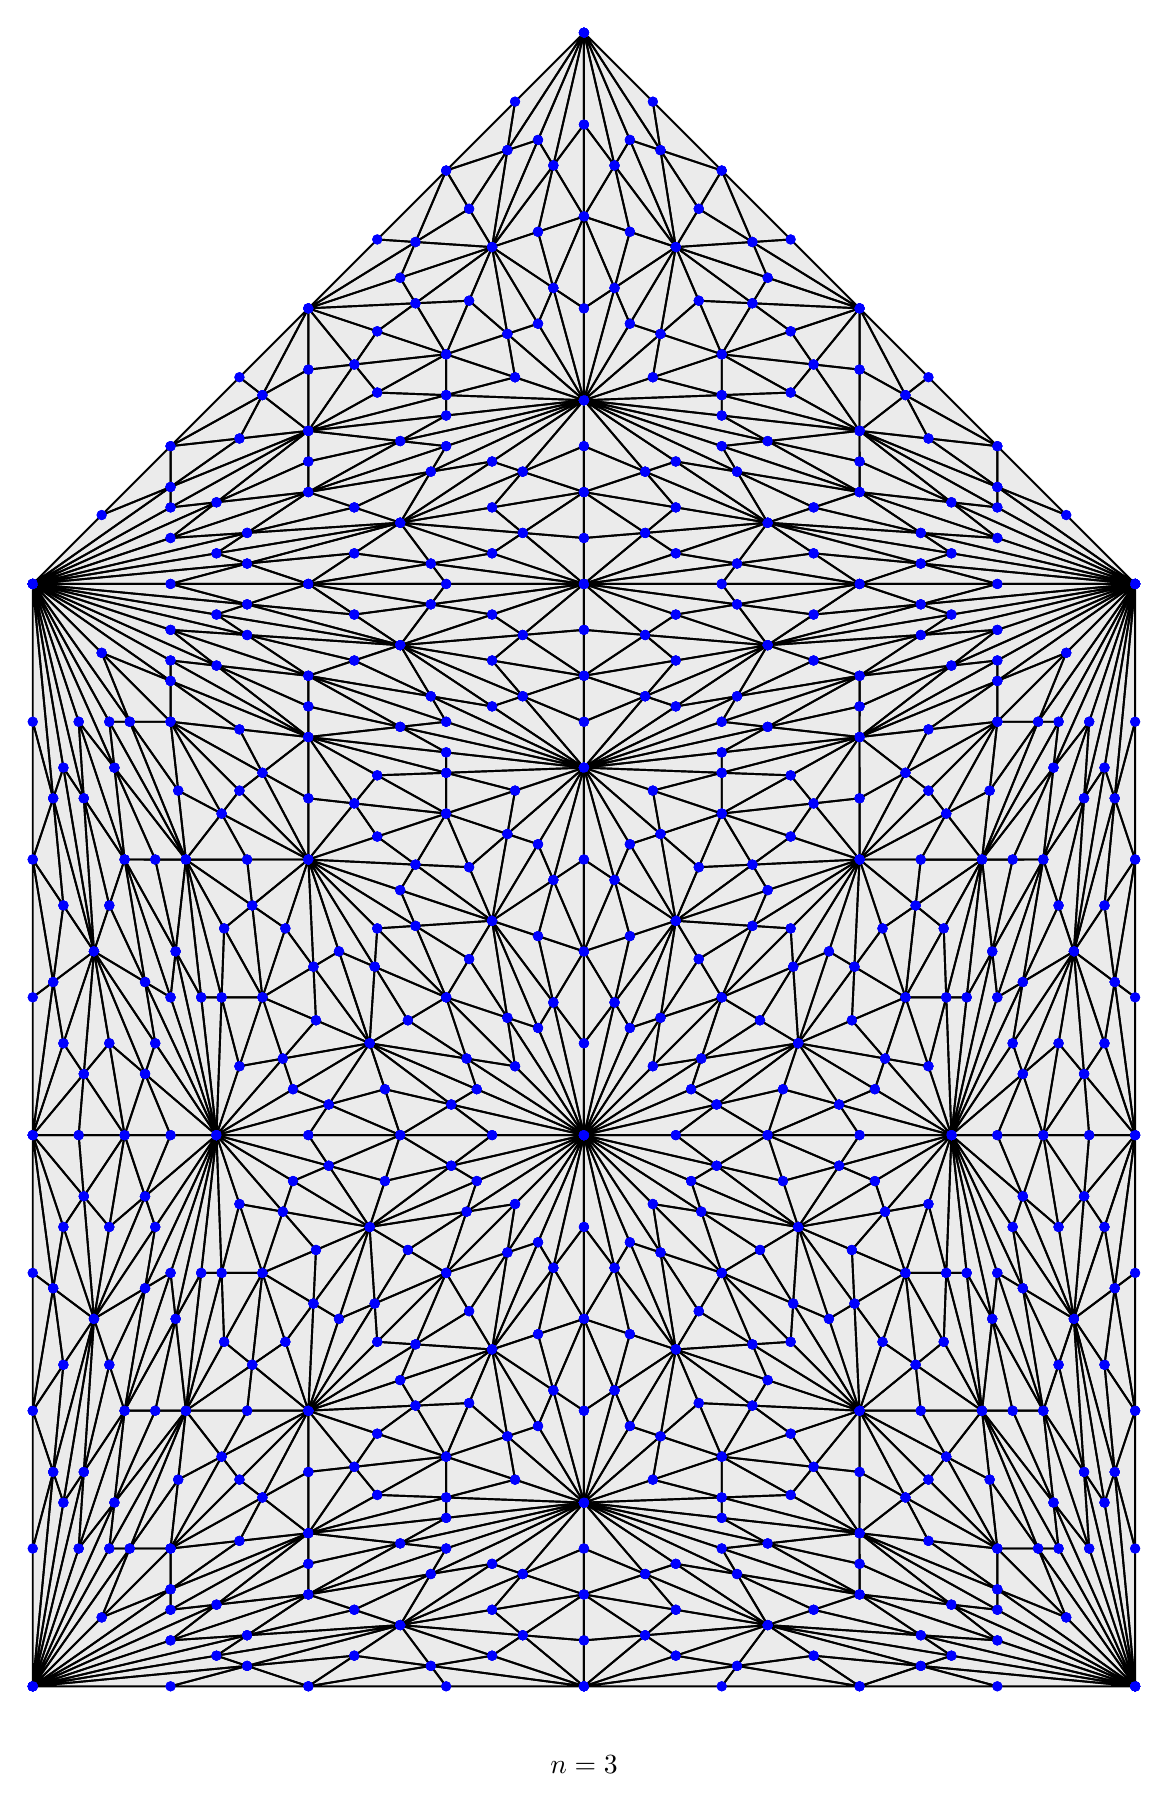
\begin{tikzpicture}
        \nikolausresidenz{3}
        \path (7,-1) node {$n=3$};
    \end{tikzpicture}
\end{center}

\end{document}
